\documentclass[8pt, letterpaper]{report}

% used for change the geometry/layout of the document
\usepackage{geometry}
\geometry{top=2.5cm, bottom=2.5cm, left=2.5cm, right=2.5cm}

% used for colored box
\usepackage{tcolorbox}

% used for import images
\usepackage{graphicx}
\graphicspath{ {./images/} }

% used for import hyperlinks
\usepackage[hidelinks]{hyperref}
\hypersetup{
    colorlinks=false, %set true if you want colored links
    linktoc=all,     %set to all if you want both sections and subsections linked
    linkcolor=blue,  %choose some color if you want links to stand out
}

% used for import font colors
\usepackage{xcolor}

% used to read the file name
\usepackage{currfile}




\usepackage{lastpage}
\usepackage{fancyhdr}
\pagestyle{fancy} 


\fancyhead{} % remove the header shitty line


%\chead{\begin{picture}(0,0) \put(0,0){
\includegraphics[width=2cm]{Logo}} \end{picture}}
% \chead{
\includegraphics[width=\textwidth,height=\textheight,keepaspectratio]{Logo}}
\cfoot{\thepage\ of \pageref{LastPage}}
\lfoot{\today\newline\currfilename}
\rfoot{LIEBHERR MACHINE BULLE}


\renewcommand{\headrulewidth}{2pt}% Default \headrulewidth is 0.4pt

% Redefine the plain page style
\fancypagestyle{plain}{}


\begin{document}

\author{AC22}




\title{{\vspace{-10.0cm}{\textsc{Manual}\\Result Viewer}}}
\maketitle
\tableofcontents
\clearpage


\chapter{Read}

Read TestResult from the Reading folder is possible via the following command:
\\\\
Toolbar \textrightarrow 
\includegraphics{Read}\\
Menu \textrightarrow \textbf{File/Read}
\\\\\\
Because of speed performance, only N last generated files will be readed. is possible to set this value from the number input widget
\\
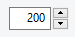
\includegraphics{NumberOfTest}.
\\\\
The reading folder can be reset to the default folder using the following command:
\\\\
Toolbar \textrightarrow 
\includegraphics{ResetFolder}\\
Menu \textrightarrow \textbf{File/Reset folder}

\clearpage
\chapter{View}

To view the TXT or HTML version of TestResult/s selected. Right click on the list of result, click the preferred option from the context menu.
\\\\
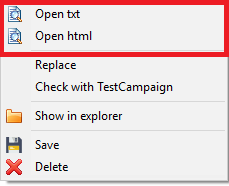
\includegraphics{contextMenu}
\\\\
From the context menu is also possible to:\\
- Replace in one or multiple TestResult, one specific field with a choosen value.\\
- Open the folder of selected TestResult.\\
- Save selected TestResult.\\
- Delete selected TestResult.\\

\clearpage
\chapter{Filtering}

Is possible to filter the visualized result using the toolbar filter widget.\\
Select the column you want to filter, type the string to filter and click [ENTER] to refresh the list.
\\\\
\includegraphics[width=\textwidth,height=\textheight,keepaspectratio]{Filter_toolbar}
\\\\
Reset filter is possible via menu \textbf{Filter/Reset all}.\\
Is possible to check/uncheck the case sensitive via menu \textbf{Filter/Case sensitive}.\\
From the Filter menu is possible to set quick filters.

\clearpage
\chapter{Save}

To save the selected TestResult to the Saving folder use the following command:
\\\\
Toolbar \textrightarrow 
\includegraphics{Save}\\
Menu \textrightarrow \textbf{File/Save}\\
Context menu \textrightarrow  \textbf{Save}
\\\\
If TestResult is linked with one or more MDF file/s, the MDF/s is/are saved as well in the saving folder.


\clearpage
\chapter{Report}



\section{Read Test Result} 
The report is generated using the test result displayed on the ResultViewer list.
\begin{itemize}  
\item Update SVN Folder containing test result
\item Read folder (Menu \textbf{File/Read})l
 \begin{tcolorbox}[colframe=white!100!black, colback=red!50!white, sharp corners=all]
 \textbf{Attention}\\
Request at least 1000 test cases and check that the number of test is below 1000
\end{tcolorbox}
\item Check there are no error messages in the dedicate box
\item Correct all problems
\item Commit SVN Folder after modifications
\end{itemize}

\clearpage


\section{Create Excel/PDF}




\subsection{Summary file}
Open the template of Test Report Summary\newline
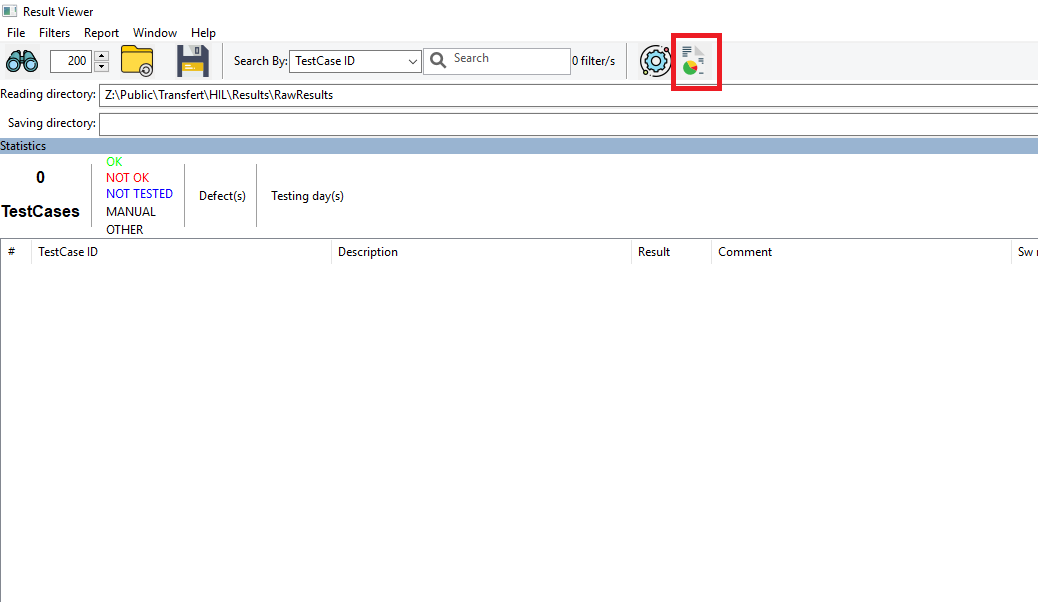
\includegraphics[width=\textwidth,height=\textheight,keepaspectratio]{OpenTestReport}
\newline
\newline
Fill the page with correct information\newline
Save the document to your PC. Change file name to match your Validation\newline
Example : LMB\_AC\_48\_\textcolor{red}{XXXX}\_TestSummaryReport \textcolor{red}{24.13.10 236901 BETA PEGASUS D956}.xlsx\newline
\newline






\subsection{Generate Result}
Start the generation process via menu \textbf{Report/Generate (Excel)}.
 \begin{tcolorbox}[colframe=white!100!black, sharp corners=all]
 \textbf{Note}\\
Overview, Traceability, Incident checkboxes from Report menu must be activated.
\end{tcolorbox}
Open the Summary excel file previously created.\newline
Move the recently created sheets (Result, Traceability, Incident) inside the Validation Report at the end of it.\newline
\newline
Define "Print Area"
\begin{itemize} 
	\item Select column A to I
	\item Go in Page Layout Menu and Select Print Area
	\item Click Set Print Area
\end{itemize} 
Define "Page Break Preview" to print on one page
\begin{itemize} 
	\item Go in View Menu and Select Page Break Preview
	\item Slide dotted line to the end of clolumn I
\end{itemize} 

If all test are green, Approve the report, else don't approve it\newline
\newline
Fill in the AC22 Comment part by highlighting each topic on which deviations are observed and by referring the "Result" Sheet\newline
\newline








\subsection{Review}
Send report by mail for review and to fill dedicated field to Malnoy + Lescot + Rimkus + CSM (if exist)








\subsection{Wait}
Wait for request to start workflow (from AC1 or CSM)




\subsection{Save as PDF}
Open the Test report.\newline
Correct page setup\newline
- Pages ResultAssessment: choose function file/print/Fit All columns on One Page\newline
Export document as PDF\newline
- ALL THE PAGES OF THE EXCEL REPORT MUST BE IN THE PDF\newline

\clearpage


\section{Create HTML}
Display the Test Result of which you want to generate the report.\newline
Start the generation process via menu \textbf{Report/Generate (HTML)}.
Report is generated in same folder choose to display the Test Result.\newline

\subsection{Add on}
Add on files can be used to add content to the final report without worrying about style.

 \begin{tcolorbox}[colframe=white!100!black, colback=red!50!white, sharp corners=all]
 \textbf{Attention}\\
Content of Add on will be automatically added to the report only if they are present in the same folder where the report is generated.
\end{tcolorbox}
Following table will give a short description of each add on:\newline
\newline
\resizebox{\textwidth}{!}{%
	\begin{tabular}{ | c | c | c |}
	\hline
	\textbf{Add on} & \textbf{Description} & \textbf{Responsible}\\ 
	\hline
	 Info & Add to the Summary page the information about the maturity and project of the SW under test. & AC22\\ 
	 \hline
	 Deviation & Allow CSM + AC to give a status for each deviation raised during the validation of SW. & CSM + AC\\
	 \hline
	\end{tabular}
}
\clearpage



\section{ISO number}
Copy end of the file name : TestSummaryReport 24.13.10 236901 BETA PEGASUS D956\newline
Go here : \href{https://lmbweb.liebherr.i/team/WS5/Team/ISOdoc/default.aspx}{\textcolor{blue}{https://lmbweb.liebherr.i/team/WS5/Team/ISOdoc/default.aspx}}
\begin{itemize} 
\item Click on New item
\item Paste Document Name
\item Chose document type 48 - Test Summary
\item Click Submit
\item Click Get Number - Click a second time if number does not appear yet
\item Add the ISO number in file name : LMB\_AC\_48\_1136\_TestSummaryReport 24.13.10 236901 BETA PEGASUS D956.xlsx
\end{itemize} 

\clearpage


\section{Save to Sharepoint}
\href{https://lmbweb.liebherr.i/team/WS5/Team/Release/Hil\%20Test\%20Reports/Forms/AllItems.aspx}{\textcolor{blue}{Link}} to reports folder.\newline
Select the appropriated ECU type folder.\newline
- Go in the Root directory of your software : ex. 24.13.10\newline
- Create your SW folder XXXXXX\_YYY\newline
- XXXXXX is the SVN revision of the SW\newline
- YYY is the SW type ALPHA/BETA/RC/RTM\newline
- Add and check in your document in the folder\newline

\clearpage


\section{Workflow}
Open the Test report in Sharepoint\newline
Launch Workflow \textrightarrow Report approval by AC \textrightarrow  Start\newline
You will receive an email\newline
Click on it and add Malnoy + Wallmueller + Rimkus + CSM (if exist)\newline


\clearpage


\end{document}